\section{Analysis for \cref{sec:fft}}
\label{app:sfft-details}
\subsection{Additional Details}\label{app:ssec:fft-additional-definitions}

\mypar{Defining the circulant matrix}
We consider the special case where $\bfA$ is the prefix sum linear query matrix (lower-triangle matrix of ones). Then, we define the corresponding circulant matrix
\begin{equation}
    \acirc\triangleq\begin{bmatrix}
        v_0 & v_{2n-1} & \cdots & v_1\\
        v_1 & v_0 & \cdots & v_2\\
        \vdots & \vdots & \cdots & \vdots\\
        v_{2n-1} & v_{2n-2} & \cdots & v_0
\end{bmatrix}
\qquad \text{where} \qquad
\bfv \triangleq [\underbrace{1,\ldots,1}_{n},\underbrace{0,\ldots,0}_{n}].
\label{eq:circRep}
\end{equation}
It is straightforward to verify ${\acirc}\idx{:n}{:n} = \bfA$.

\mypar{Defining the DFT}
\begin{equation}
    \forall k\in[2n-1]: \fexd[k]=\sum\limits_{a=0}^{2n-1}\bfv(a)\exp\left(\frac{-j2\pi k a}{2n}\right)
    \label{eq:DFT}
\end{equation}

\mypar{Circulant matrices expressed using Fourier Transforms}
\begin{thm}[Adapted from~\cite{gray2006toeplitz}]
    Consider any circulant matrix $\acirc\in\mathbb{R}^{2n\times 2n}$. Let $\fft\in\mathbb{C}^{2n\times 2n}$, where the $k$-th row of $\fft$ is given by  $\fft[k,:]=\frac{1}{\sqrt{2n}}\left[\exp\left(-\frac{j2\pi ka}{2n}\right):a\in\{0,\ldots,2n-1\}\right]$. Then, $\acirc=\fft^{\herm}\Sigma\fft$, where $\Sigma\in\mathbb{C}^{2n\times 2n}$ is a diagonal matrix with the diagonal being the DFT (defined in~\Eqref{eq:DFT}) of the first column of $\acirc$. Here, $\herm$ is the Hermimitian operation.
    \label{thm:circDiag}
\end{thm}

\mypar{Privacy and utility guarantees} In the following we provide the privacy guarantee and the main utility guarantee  for the FFT mechanism defined in Algorithm~\ref{alg:fft}.
\begin{thm}[DP-Prefix Sum via FFT Privacy Guarantee]
Algorithm~\ref{alg:fft} is $\rho$-zCDP in the adaptive continuous release model.
\label{thm:privFFT}
\end{thm}
Next, we analyze the utility of Algorithm~\ref{alg:fft} and show that it is nearly optimal in terms of the mean squared error (MSE) in the single-pass setting. First, we express the MSE in Theorem~\ref{thm:MSE} below.
\begin{thm}[DP-Prefix Sum via DFT Utility]
The MSE achieved by Algorithm~\ref{alg:fft} using the real and imaginary components of $\widetilde\bfz$ is
$$\mathbb{E}\left[\mse\right]=\frac{\kappa^2\lone{\fexdt}^2}{2\rho n^2}.$$
\label{thm:MSE}
\end{thm}
In the following, we will have an explict expression for $\lone{\fexdt}$ in terms of the problem parameters. Finally, we will argue that Theorem~\ref{thm:MSE} is nearly optimal.


\begin{cor}
The expected mean squared error (MSE) is given by the following:
$$\mathbb{E}\left[\mse\right]=\frac{\kappa^2}{2\rho n^2}\left(n+\sum\limits_{a=0}^{\lfloor\frac{2n-1}{2}\rfloor}\frac{1}{\sin\left(\frac{\pi(2a+1)}{2n}\right)}\right)^2.$$
\label{cor:mse}
\end{cor}





\vspace{-1em}
\mypar{Near-optimal utility} Here, we show that Theorem~\ref{thm:MSE} is near-optimal in utility for the single-participation setting.
To do this, we compare with a lower bound on the expected $\mse$ of any factorization-based mechanism
from~\citet[Theorem 2]{HUU22}: $\frac{1}{2\rho\pi^2}\left(2+\ln\left(\frac{2n+1}{3}\right)+\frac{\ln(2n+1)}{2n}\right)^2$. We find that the though our analytical upper bound in Corollary~\ref{cor:mse} is $\approx6$x worse than the lower bound, the empirical noise added in Algorithm~\ref{alg:fft} closely tracks the lower bound to within a factor of $1.2$x---because it only adds the real part of the noise. Results are in Figure~\ref{fig:lbc} of Appendix~\ref{app:ssec:fft-additional-definitions}.

\textbf{Showing near-optimal utility via MSE experiments}
\FloatBarrier  %

\begin{figure}[H]
    \vspace{-4mm}
    \centering
    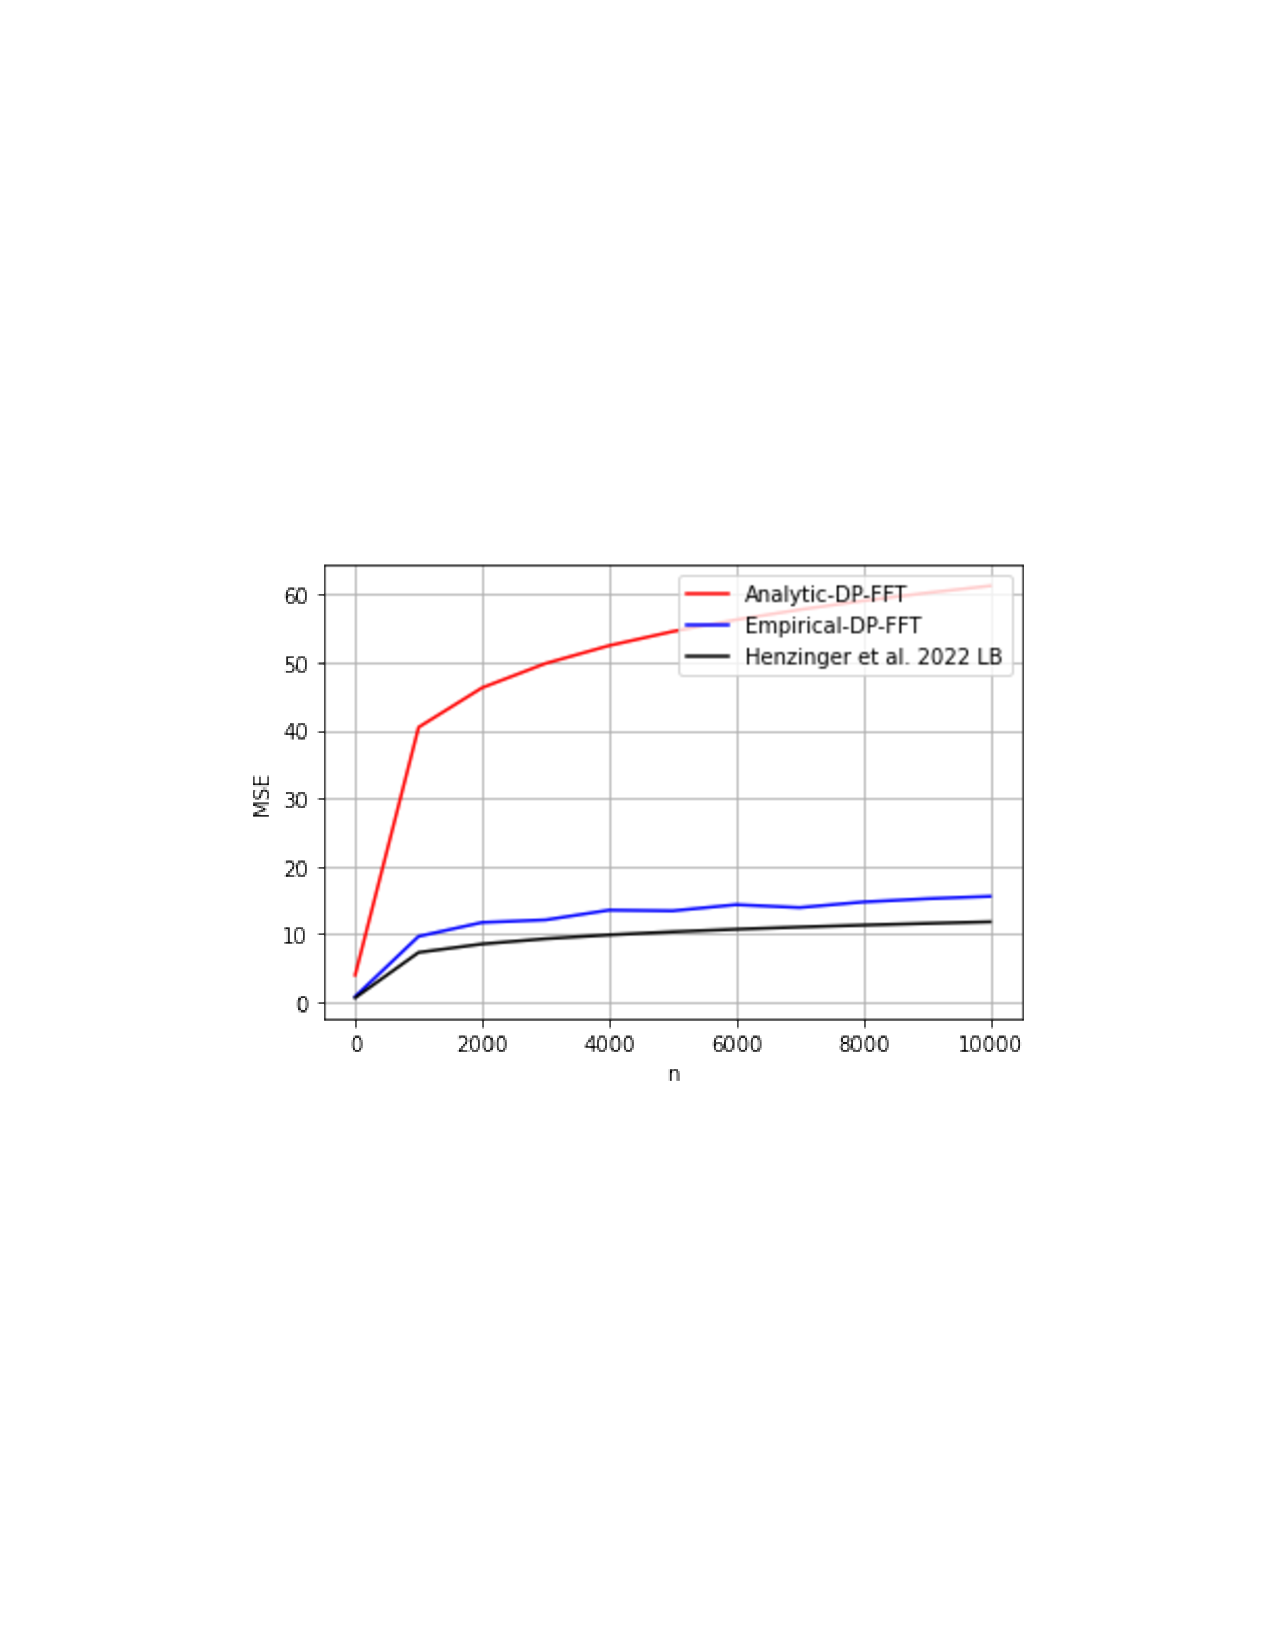
\includegraphics[trim={4.25cm 9cm 4cm 9cm},clip,scale=0.5]{icml2023/figures/lb_comp/lb_comparison.pdf}\vspace{-6mm}
    \caption{\textbf{Algorithm~\ref{alg:fft} achieves near-optimal utility} as measured by the analytic lower bound from~\citet[Theorem 2]{HUU22}.}
    \vspace{-1em}
    \label{fig:lbc}
\end{figure}

\subsection{Proof of~\cref{thm:privFFT}}\label{app:ssec:privFFT}
\begin{namedtheorem}[\cref{thm:privFFT}]
Algorithm~\ref{alg:fft} is $\rho$-zCDP in the adaptive continuous release model.
\end{namedtheorem}
\begin{proof}
First, consider the non-adaptive setting and the following mechanism, with parameters as defined in Algorithm~\ref{alg:fft},
\begin{align}
 \left[\Sigma\left(\fft\exd+\Sigma^{-1}\bfz\right)\right],\nonumber\\  \text{where $\bfz=\sqrt{\frac{\kappa^2\lone{\fexdt}}{4n\rho}}\left(\sqrt{\Sigma}\cdot\bfw\right)$}  
 \label{eq:factmech1}
\end{align}
We claim that this satisfies $\frac{\kappa^2\lone{\fexdt}}{4n\sigma^2}$-zCDP. To see this, we proceed by bounding $\rho_i$ for each coordinate $i \in [2n]$ defined in~\Eqref{eq:factmech1}. 
For brevity, let $\bfb=\fft\exd$. Consider two neighboring data sets $\bfg$ and $\bfg'$, correspondingly, $(\bfb,\exd)$ and $(\bfb',\exd')$. Then,
\begin{equation}
    \linfty{\bfb-\bfb'}=\linfty{\fft(\exd-\exd')}=\frac{\kappa}{\sqrt{2n}}.\label{eq:sens}
\end{equation}
We will now prove zCDP guarantee independently for each of the $2n$ coordinates and then use standard zCDP composition~\citep{bun2016concentrated}. For any coordinate $a\in\{0,\ldots,2n-1\}$, adding noise $\left(\frac{\sigma}{\sqrt{|\fexd[i]|}}\right)\cdot \calN_{\sf complex}\left(0,1\right)$ to $\bfb[i]$ satisfies $\rho_i$-zCDP with $\rho_i=\frac{\kappa^2|\fexd[i]|}{4n\sigma^2}$. Then by composition, we have that
\begin{equation}
    \rho = \sum\limits_{a=0}^{2n-1} \left(\rho_i\right)=\frac{\kappa^2}{4n\sigma^2}\sum\limits_{a=0}^{2n-1}\left(\left|\fexd[i]\right|\right)=\frac{\kappa^2\lone{\fexdt}}{4n\sigma^2}.
    \label{eq:zCDPtot}
\end{equation}
Therefore, setting $\sigma^2=\frac{\kappa^2\lone{\fexdt}}{4n\rho}$-satisfies a non-adaptive $\rho$-zCDP. Using the same $\sigma$, we prove the adaptive part using the same $\sigma$. We have the following from~\Eqref{eq:factmech1}.
{\small
\begin{equation}
    \hspace{-2.5mm}\left[\fft\herm\left(\Sigma\fft\exd+\bfz\right)\right]=
    \left[\fft\herm\sqrt{\Sigma}\left(\sqrt{\Sigma}\fft\exd+\frac{1}{\sqrt{\Sigma}}\bfz\right)\right]=
    \left[\fft\herm\sqrt{\Sigma}\left(\sqrt{\Sigma}\fft\exd+\sqrt{\frac{\kappa^2\lone{\fexdt}}{4n\rho}}\cdot\bfw\right)\right]
    \label{eq:0uf}
\end{equation}}
Since, $\bfw$ in~\Eqref{eq:0uf} is spherical Gaussian, and the original query matrix $\bfA$ is lower triangular, by Theorem 2.1 in~\citet{denisov22matfact}, the adaptive privacy guarantee follows.
\end{proof}

\subsection{Proof of~\cref{thm:MSE}}\label{app:ssec:MSE}
\begin{namedtheorem}[\cref{thm:MSE}]
The MSE achieved by Algorithm~\ref{alg:fft} using the real and imaginary components of $\widetilde\bfz$ is
$$\mathbb{E}\left[\mse\right]=\frac{\kappa^2\lone{\fexdt}^2}{2\rho n^2}.$$
\end{namedtheorem}
\begin{proof}
The MSE is given by the following: 
\begin{equation}
    \mathbb{E}[\mse]=\frac{1}{n}\mathbb{E}\left[\ltwo{\actnoise[0,\ldots,n-1]}^2\right]=\frac{\kappa^2\lone{\fexdt}}{2n^2\rho}\cdot\tr\left(|\Sigma[:n,:n]|\right)=\frac{\kappa^2\lone{\fexdt}^2}{2n^2\rho}.
    \label{eq:tr1}
\end{equation}
In~\eqref{eq:tr1}, $\Sigma[:n,:n]$ refers to the top-left $n\times n$ submatrix of $\Sigma$.
\end{proof}

\subsection{Proof of~\cref{cor:mse}}\label{app:ssec:mse}
\begin{namedcorollary}[\cref{cor:mse}]
Under the same setting as Theorem~\ref{thm:MSE}, the MSE for Algorithm~\ref{alg:fft} is the following
$$\mathbb{E}\left[\mse\right]=\frac{\kappa^2}{2\rho n^2}\left(n+\sum\limits_{a=0}^{\lfloor\frac{2n-1}{2}\rfloor}\frac{1}{\sin\left(\frac{\pi(2a+1)}{2n}\right)}\right)^2.$$
\end{namedcorollary}

\begin{proof}
Recall the definition of DFT from~\Eqref{eq:DFT} and of $\bfv$ in~\Eqref{eq:circRep}. It is immediate that $\fexd[0]=n$. For any $k\neq 0$, we have,
\begin{equation}
    \fexd[k]=\frac{1-\exp\left(\frac{-j2\pi k n}{2n}\right)}{1-\exp\left(\frac{-j2\pi k}{2n}\right)}=\frac{1-\exp\left({-j\pi k }\right)}{1-\exp\left(\frac{-j\pi k}{n}\right)}.
    \label{eq:f2}
\end{equation}
From~\Eqref{eq:f2}, we have that when $k>0$ is even, $\fexd[k]=0$. For $k$ odd, we have
\begin{equation}
    \left|\fexd[k]\right|=\left|\frac{2}{1-\exp\left(\frac{-j\pi k}{n}\right)}\right|=\frac{1}{\left|\sin(\pi k/(2n))\right|}=\frac{1}{\sin(\pi k/(2n))}
    \label{eq:f3}
\end{equation}
Combining these, the term $\lone{\fexdt}$ is
\begin{equation}
    \lone{\fexdt}=n+\sum\limits_{a=0}^{\lfloor\frac{n-1}{2}\rfloor}\frac{1}{\sin(\pi(2a+1)/(2n))}
\end{equation}
\end{proof}

\subsection{Proof of~\cref{thm:multip}}\label{app:ssec:multip}
\begin{namedtheorem}[\cref{thm:multip}]
Under $\maxpart$ participation, Algorithm~\ref{alg:fft} satisfies $(\maxpart^2\rho)$-zCDP.
\end{namedtheorem}
\begin{proof}
The proof goes exactly as Theorem~\ref{thm:privFFT}, except~\eqref{eq:sens} gets replaced by the following:
\begin{equation}
    \linfty{\bfb-\bfb'}=\linfty{\fft(\exd-\exd')}=\frac{\maxpart\kappa}{\sqrt{2n}}.\label{eq:sensx}
\end{equation}
\end{proof}




